\documentclass[fleqn]{article}
\usepackage[nodisplayskipstretch]{setspace}
\usepackage{amsmath, nccmath}
\usepackage{amssymb}
\usepackage{enumitem}
\usepackage{etoolbox}
\usepackage{graphicx}
\usepackage{float}
\usepackage{changepage}
\usepackage{environ,capt-of}

\newcommand{\zerodisplayskip}{
	\setlength{\abovedisplayskip}{0pt}%
	\setlength{\belowdisplayskip}{0pt}%
	\setlength{\abovedisplayshortskip}{0pt}%
	\setlength{\belowdisplayshortskip}{0pt}%
	\setlength{\mathindent}{0pt}}
	
\makeatletter
	\newenvironment{equationCenter}{\@fleqnfalse\begin{equation*}}{\end{equation*}}
\makeatother

\let\oldfigure\figure% Store original figure float environment
\let\endoldfigure\endfigure
\RenewEnviron{figure}[1][H]{% Update figure environment
  %\par\vspace{\intextsep}% Assume in-text placement, so insert appropriate vertical spacing
  \noindent
  % \patchcmd{<cmd>}{<search>}{<replace>}{<success>}{<failure>}
  \patchcmd{\BODY}{\caption}{\captionof{figure}}{}{}% Replace \caption with \captionof{figure} inside \BODY
  % Set "figure"
  \begin{minipage}{\linewidth}
    \BODY
  \end{minipage}
  %\par\vspace{\intextsep}% Assume in-text placement, so insert appropriate vertical spacing
}

\title{Homework 6}
\author{Owen Sowatzke}
\date{November 21, 2023}

\begin{document}
	\offinterlineskip
	\setlength{\lineskip}{12pt}
	\zerodisplayskip
	\maketitle
	\begin{enumerate}
		\item Let's use the frequency sampling method to design a causal, symmetric FIR lowpass filter. Consider the following ideal frequency response (assumed to be periodic with period $2\pi$):
		
		\begin{equationCenter}
			H(e^{j\omega}) = \begin{cases}
				1 & \text{for}\ |\omega| < \omega_c\\
				0 & \text{for}\ 0 \leq |\omega| \leq \pi
			\end{cases}
		\end{equationCenter}
		
		In the frequency sampling method, we sample this ideal frequency response as follows:
		
		\begin{equationCenter}
			H(k) = H(e^{j\omega_k})\ \text{for}\ k = 0,1,...,N-1
		\end{equationCenter}
		
		where $\omega_k = 2{\pi}k/N$. Then we calculate a zero-phase filter as $h(n) = \text{IDFT}\{H(k)\}$ for $n = 0,1,...,N-1$. Finally, we rearrange the samples to obtain a causal filter.
		
		\begin{enumerate}[nolistsep]
			\item Let $N = 16$. Our goal is to have the cutoff frequency be $\omega_c = 0.5\pi$ such that $H(e^{j0.5\pi}) = \sqrt{2}/2 = 0.7071$. Use MATLAB (or Python or C) to create a 16-element \texttt{H} array containing mostly ones and zeros arranged in such a way that they correspond to the above equation for $H(k)$. You'll have to be careful with array indexing since the MATLAB array index starts at 1 instead of 0. Initialize the array contents to begin with ones for the passband ($0 \leq \omega < \omega_c$), followed by zeros for the stopband ($\omega_c < \omega < 2\pi - \omega_c$), followed by ones for the the passband ($2\pi - \omega_c < \omega < 2\pi$). At the two array indexes that correspond to the cutoff frequency, use transition samples with value 0.7071. Plot the \texttt{H} array.
			
			\begin{figure}[H]
				\centerline{\fbox{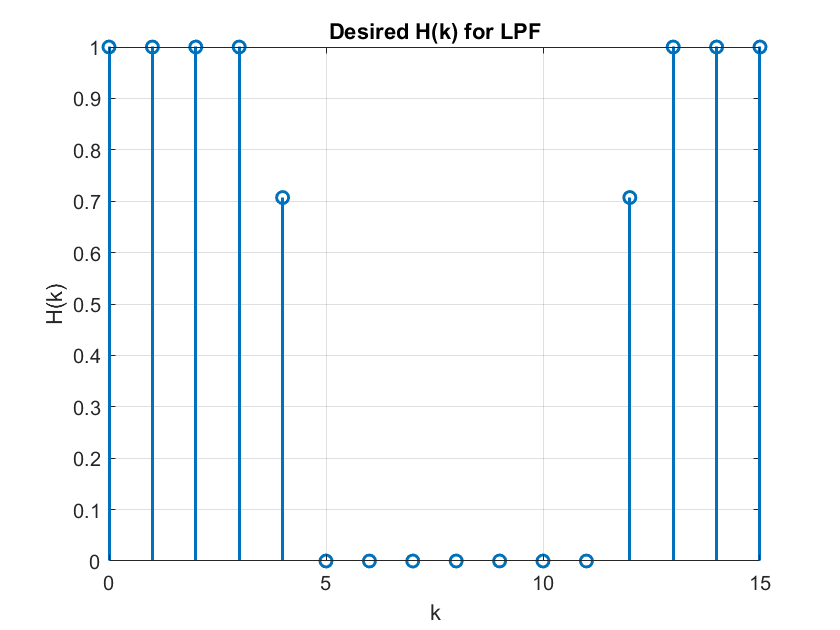
\includegraphics[width=0.5\textwidth]{prob1a_array_H.png}}}
				\caption{Plot of the Values in the Array \texttt{H}}
			\end{figure}
			
			\item Compute the inverse DFT using \texttt{h = ifft(H)}. Show the values you obtain. Since $H(e^{j\omega})$ and $H(k)$ are real and even in the equations above, we expect that the imaginary part of the inverse FFT should be approximately zero. Plot the resulting \texttt{h(n)} for \texttt{n = 0} to \texttt{15}. For example, in MATLAB you can do \texttt{n = 0:15; stem(n,h)}.
			
			\begin{figure}[H]
				\centerline{\fbox{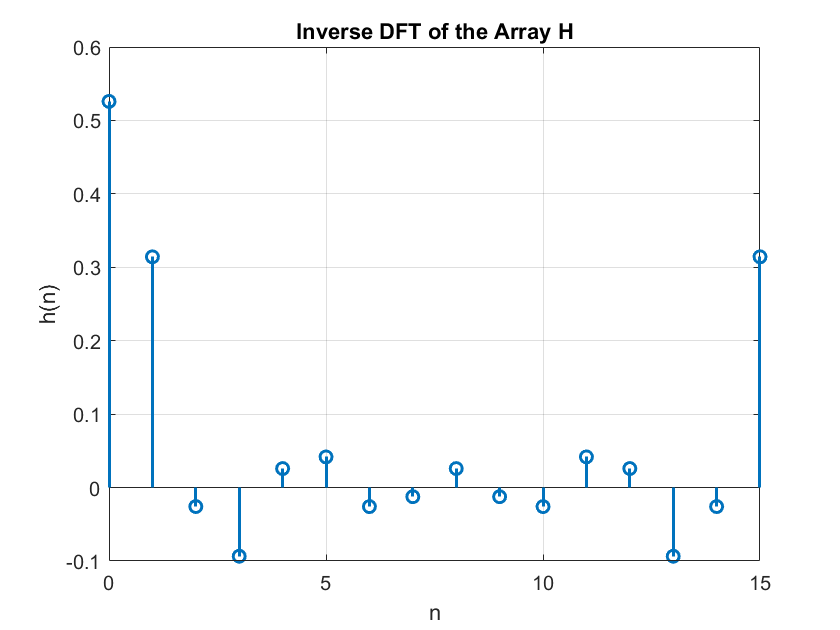
\includegraphics[width=0.5\textwidth]{prob1b_ifft_of_H.png}}}
				\caption{Inverse DFT of the Array \texttt{H}}
			\end{figure}
			
			\pagebreak
			\item Using 16 samples over $0 \leq \omega < 2\pi$, plot the frequency response. For example, in MATLAB:
			
			\texttt{H = fft(h);}
			
			\texttt{stem(abs(H))}
			
			How does this plot compare to the ideal frequency response?
			
			\begin{figure}[H]
				\centerline{\fbox{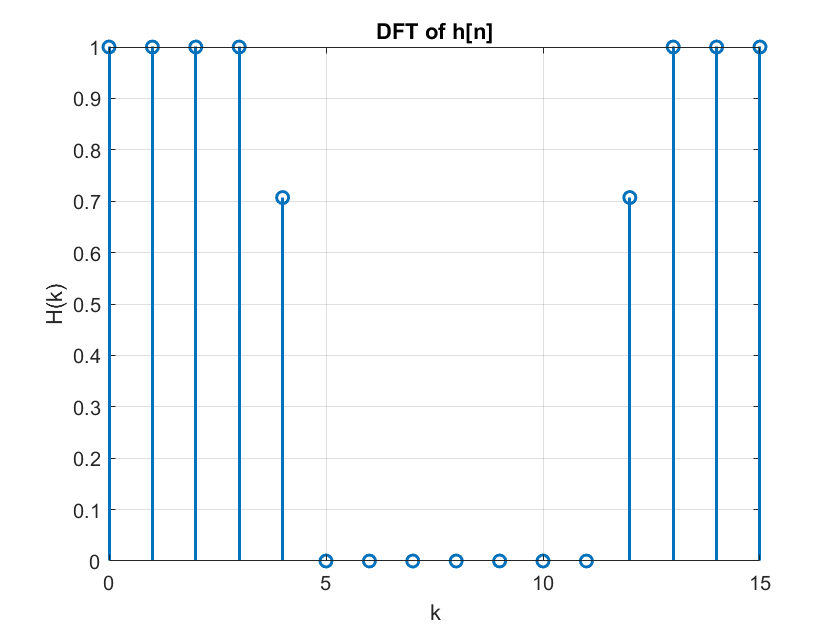
\includegraphics[width=0.5\textwidth]{prob1c_freq_response.png}}}
				\caption{DFT of $h[n]$}
			\end{figure}
			
			Note that the frequency response matches the ideal frequency response exactly at each of the frequencies samples we specified when defining $H(k)$.
			
			\item Rearrange the elements of \texttt{h} to obtain a causal, symmetric impulse response, \texttt{hc}. Plot the result. For example, in MATLAB do \texttt{stem(hc)}. What is the final length of this filter?
			
			The output of the inverse DFT, \texttt{h}, is one period of the Discrete Fourier Series. The causal, symmetric impulse response will be the Discrete Fourier Series from $n=-\frac{N}{2}$ to $n=\frac{N}{2}$ with the samples at $n=-\frac{N}{2}$ and $n=\frac{N}{2}$ halved. Note that halving the endpoints is necessary if we want to prevent magnitude distortion of \texttt{H(k)}.
			 
			\pagebreak
			Consider circular shifting the array of samples, \texttt{h}, by $N/2$. The circular shift should not distort the magnitude of the DFT samples.
			
			\begin{equation*}
				h_s[n] = h[(n - N/2)\ \text{mod}\ N] \leftrightarrow H[k]e^{\frac{-j{2\pi}(N/2)k}{N}}
			\end{equation*}
			
			If we take a 2N-point DFT of $h_c[n]$, the frequency response samples that we want to match to $H[k]$ are:
			 
			\begin{equation*}
				H_c[2k] = \sum_{n=0}^{2N-1}{h_c[n]e^{-\frac{j2{\pi}n(2k)}{2N}}} = \sum_{n=0}^{2N-1}{h_c[n]e^{-\frac{j2{\pi}nk}{N}}}
			\end{equation*}
			
			\begin{equation*}
				= \sum_{n=0}^{N-1}{h_c[n]e^{\frac{-j2{\pi}nk}{N}}} + \sum_{n=N}^{2N-1}{h_c[n]e^{\frac{-j2{\pi}nk}{N}}}
			\end{equation*}
			
			\begin{equation*}
				 = \sum_{n=0}^{N-1}{h_c[n]e^{\frac{-j2{\pi}nk}{N}}} + \sum_{n=0}^{N-1}{h_c[n+N]e^{-\frac{j2{\pi}(n+N)k}{N}}}
			\end{equation*}
			
			\begin{equation*}
				 = \sum_{n=0}^{N-1}{h_c[n]e^{-\frac{j2{\pi}nk}{N}}} + \sum_{n=0}^{N-1}{h_c[n+N]e^{-\frac{j2{\pi}nk}{N}}}
			\end{equation*}
			
			\begin{equation*}
				 = \sum_{n=0}^{N-1}{(h_c[n] + h_c[n+N])e^{\frac{-j2{\pi}nk}{N}}}
			\end{equation*}
			
			Compare this to the N-point DFT of $h_s[n]$:
			
			\begin{equation*}
				H_s[k] = \sum_{n=0}^{N-1}{h_s[n]e^{\frac{-j2{\pi}nk}{N}}}
			\end{equation*}
			
			We can preserve the $H_s[k]$ samples (or the magnitude of the $H[k]$ samples) if we set:
			
			$h_c[n] + h_c[n+N] = h_s[k]$
			
			One way to do this which provides a causal filter is to let
			
			\begin{equation*}
				h_c[n] = \begin{cases}
					h_s[0]/2 & n = 0\\
					h_s[n]   & 0 < n < N\\
					h_s[0]/2 & n = N\\
					0		 & \text{otherwise}
				\end{cases}
			\end{equation*}
			
			The impulse response, $h_c[n]$, created according to the above formula is shown below:
			
			\begin{figure}[H]
				\centerline{\fbox{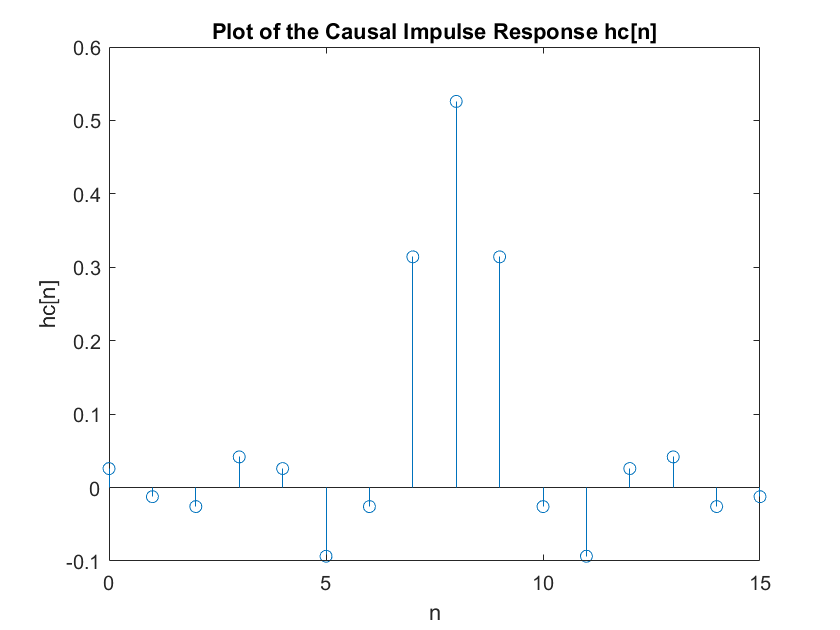
\includegraphics[width=0.5\textwidth]{prob1d_causal_impulse_response.png}}}
				\caption{Causal Impulse Response $hc[n]$}
			\end{figure}
			
			To further emphasize our selection of the causal impulse response, $h_c[n]$, we can compare $|H[k]|$ to $|H_c(e^{j\omega})|$ when the endpoints are halved and when the endpoints are not halved.
			
			\begin{figure}[H]
				\centerline{\fbox{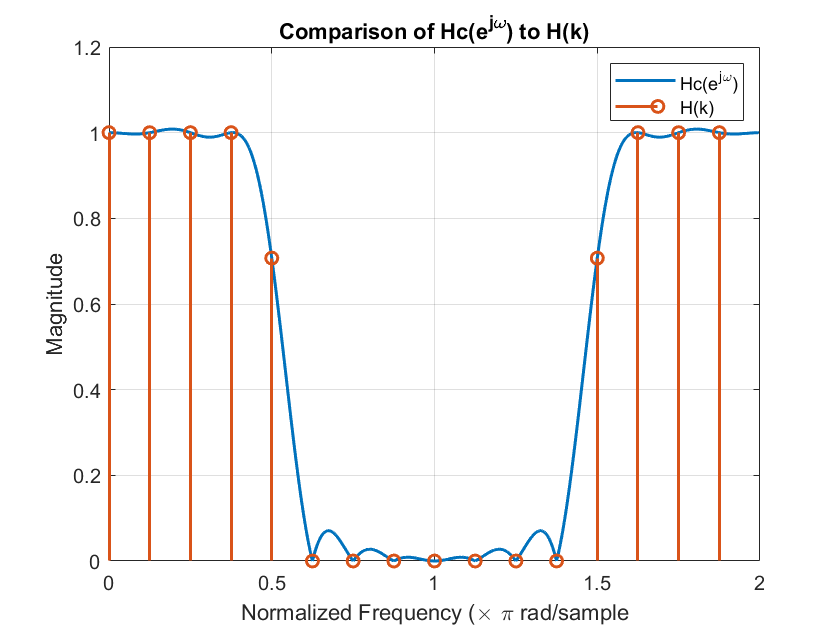
\includegraphics[width=0.5\textwidth]{prob1d_frequency_response1.png}}}
				\caption{\doublespacing Comparison of $|H(k)|$ to $|H_c(e^{j\omega})|$ when Endpoints are Halved.}
				\label{freq_response_halved_endpoints}
			\end{figure}
			
			\begin{figure}[H]
				\centerline{\fbox{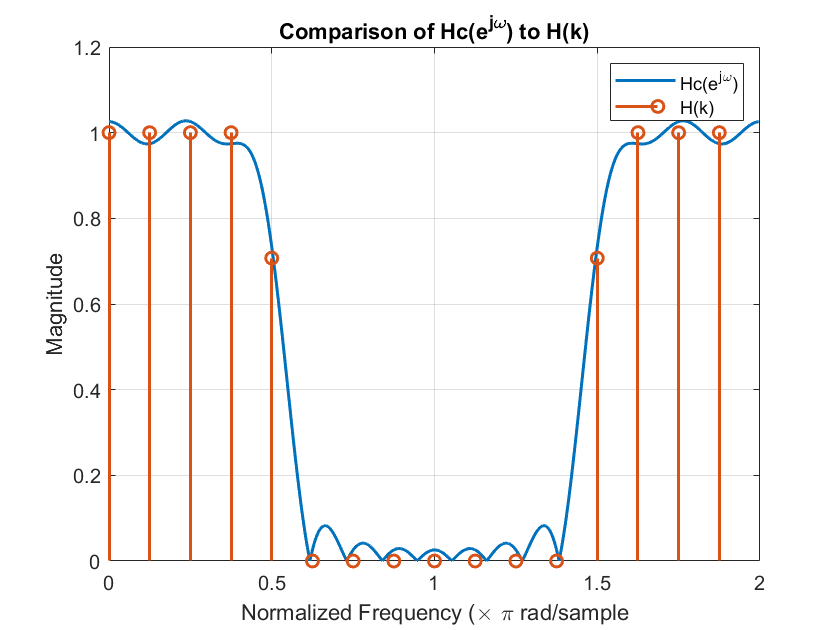
\includegraphics[width=0.5\textwidth]{prob1d_frequency_response2.png}}}
				\caption{\doublespacing Comparison of $|H(k)|$ to $|H_c(e^{j\omega})|$ when Endpoints are Not Halved.}
				\label{freq_response_raw_endpoints}
			\end{figure}
			
			Comparing, Figure \ref{freq_response_halved_endpoints} to Figure \ref{freq_response_raw_endpoints}, it is clear that halving the endpoints preserves the magnitude of the frequency response samples $H[k]$, while selecting the raw endpoints does not. Therefore, we have chosen the best option for the causal, symmetric impulse response $h_c[n]$.
			
			\item Using 512 samples over $0 \leq \omega < 2\pi$, plot the frequency response as a semilog plot. For example, in MATLAB do
			
			\texttt{[Hc,w] = freqz(hc,1,512);}
			
			\texttt{semilogy(w/pi,abs(Hc)}
			
			\texttt{axis([0 1 0.01 2]) \% lower limit 0.001 would be better}
			
			\texttt{grid on}
			
			Discuss how this plot differs the plot shown in (c).
			
			\begin{figure}[H]
				\centerline{\fbox{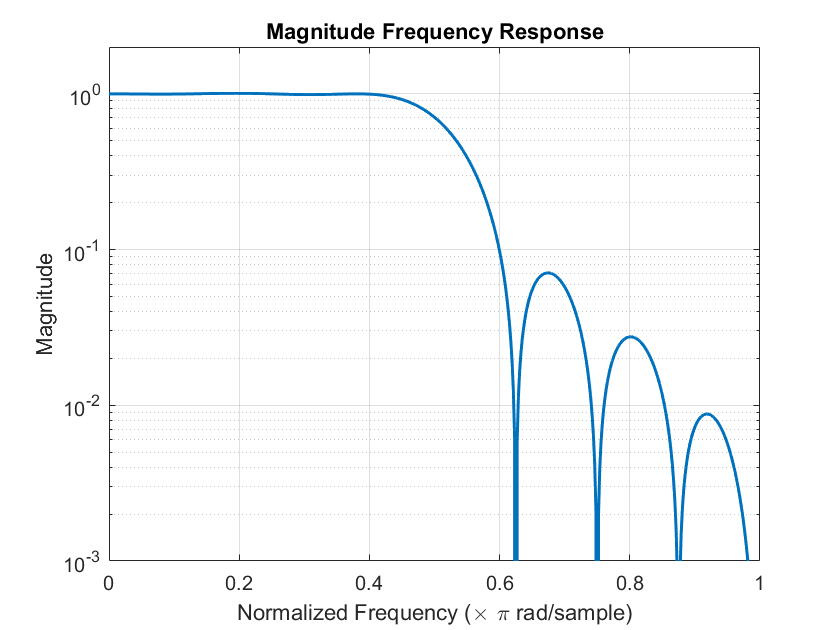
\includegraphics[width=0.5\textwidth]{prob1e_frequency_response.png}}}
				\caption{Magnitude Frequency Response.}
			\end{figure}
			
			Comparing the above figure to the plot shown in (c), we notice that it contains additional frequency response samples between those shown in part (c). Notice that the frequency response is not constant between the samples given in part (c). We see significant ripple in the stopband.
			
			\item Multiply the impulse response \texttt{hc} by a Hamming window. Then repeat (d). How do the plots differ?
			
			\begin{figure}[H]
				\centerline{\fbox{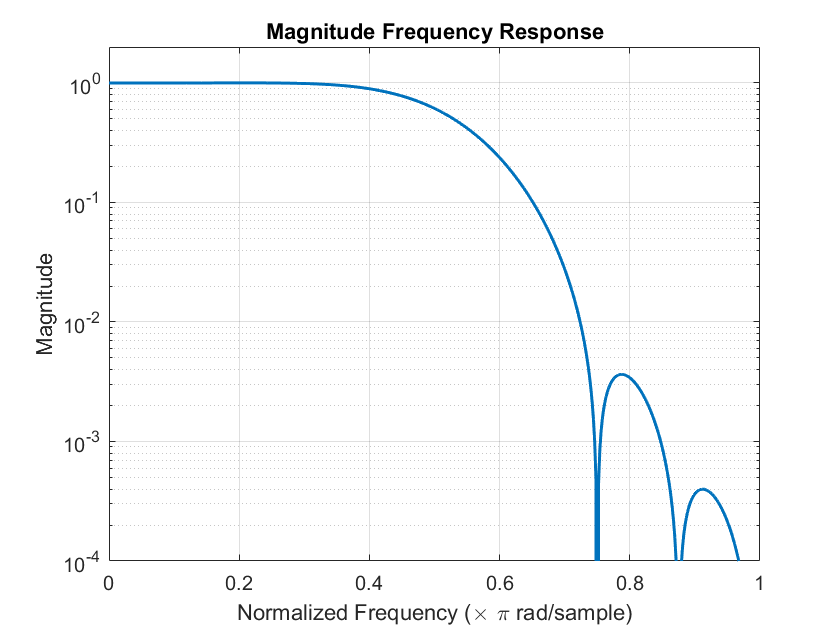
\includegraphics[width=0.5\textwidth]{prob1f_frequency_response.png}}}
				\caption{Magnitude Frequency Response.}
			\end{figure}
			
			The frequency response above has much lower sidelobes than the figure shown in part (d). However, the reduced sidelobes are not free. The frequency response shown above has a much more gradual transition between than passband and stopband than the frequency response shown in (d).
			
			\item Review the documentation for the MATLAB \texttt{fir2} function. Design an FIR LPF using the \texttt{fir2} function with length 17. Compare to the result in (f).
			
			Similar to how we designed our FIR filter, the \texttt{fir2} command takes samples of the frequency response as an input. If we provide the \texttt{fir2} function with the same frequency response samples that we used to analytically derive the impulse response, we should obtain a similar result. Note that the \texttt{fir2} command also accepts an \texttt{npt} parameter, which specifies the number of frequency samples on one side of the frequency response. This number must be greater than half the filter order. The \texttt{fir2} command internally constrains the \texttt{npt} parameter to a power of 2. If \texttt{npt} is not input as power of 2, the next power of 2 is chosen. Note that the IFFT size will be twice the \texttt{npt} parameter. To use an IFFT size that is closest to the analytic derivation, we set \texttt{npt = 16}, which results in an IFFT size of 32.
			
			The resulting command is shown below:
			
			\texttt{h = fir2(16,0:0.125:1,[1 1 1 1 sqrt(2)/2 0 0 0 0],16,0);}
			
			We can compare the \texttt{fir2} output to the impulse response we analytically derived. In the plot shown below, the impulse response output by the \texttt{fir2} command is denoted as \texttt{hm[n]}.
			
			\begin{figure}[H]
				\centerline{\fbox{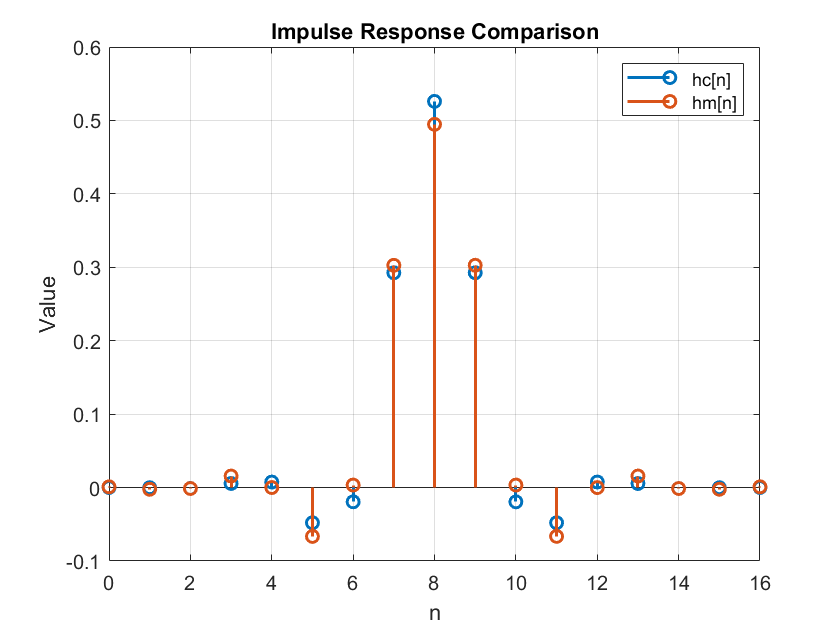
\includegraphics[width=0.5\textwidth]{prob1g_impulse_response_comparison.png}}}
				\caption{Impulse Response Comparison.}
			\end{figure}
			
			We can also compare the magnitude frequency response of both filters.
			
			\begin{figure}[H]
				\centerline{\fbox{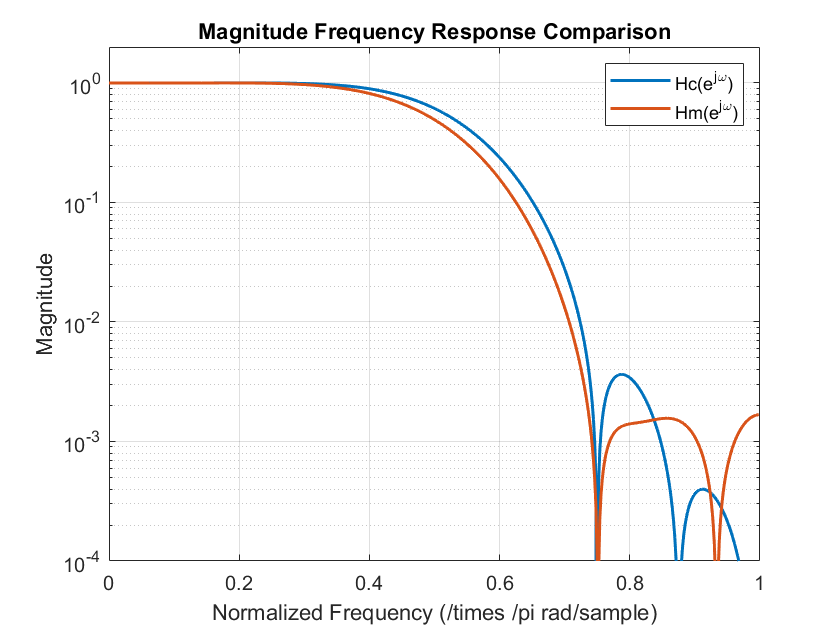
\includegraphics[width=0.5\textwidth]{prob1g_frequency_response_comparison.png}}}
				\caption{Frequency Response Comparison}
			\end{figure}
			
			Note that there are some differences in both the impulse response and frequency response. These differences arise from differences in the ideal frequency response samples. Our analytic derivation had 16 frequency response samples, while the \texttt{fir2} command used 32 frequency response samples.
			
			% If the size of the frequency response is larger than the number of specified samples, the input frequency response samples are linearly interpolated. 
			
			
		\end{enumerate}
	\end{enumerate}
	
	
	
\end{document}